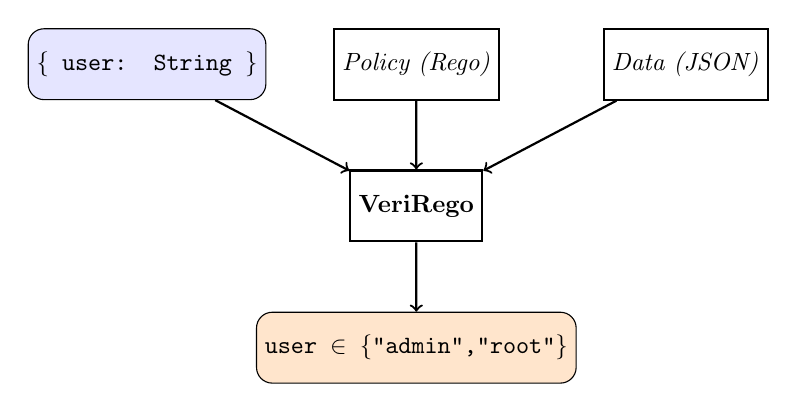
\begin{tikzpicture}[
    s/.style={draw,thick,rectangle,minimum height=10mm, minimum width=18mm},
    code/.style={draw,fill=blue!10,rectangle,minimum height=10mm, minimum width=18mm,rounded corners=2mm},
    e/.style={fill=gray!50},
    xsh/.style={xshift=15mm},
    transform shape, scale=0.9
]

    \tikzset{
        node distance=20mm,
    }

    \node[code] (input) {\texttt{\{ user: \textbf{String} \}}};
    \node[s,right of=input,xshift=18mm] (policy) {\textit{Policy (Rego)}};
    \node[s,right of=policy,xshift=18mm] (data) {\textit{Data (JSON)}};
    \node[s,below of=policy] (OPA) {\textbf{VeriRego}};
    \node[code,fill=orange!20,below of=OPA] (output) {\texttt{user $\in$ \{"admin","root"\} }};

    \draw[->,thick]
        (input) edge (OPA)
        (policy) edge (OPA)
        (data) edge (OPA)
        (OPA) edge (output)
    ;

\end{tikzpicture}
